%!TEX root = thesis.tex
\chapter{Cache Oriented Obfuscation on the System without Coherence}

In this chapter of the thesis, we proposed a method to design a reliable and efficient obfuscation technique for tightly coupled multi-processing systems by exploiting the feature of cache oriented programming. Besides, we emphasized a number of points to characterize proper attack vector. After we had elaborated our obfuscation methods and its primitives, we discussed what it is and what it is not on pitfalls and fallacies section. Finally, on the implementation section, we drew a picture of possibilities on practical applications. However, this chapter and this thesis does not concern specific and deeper studies on obfuscation and memory protection(TLB, MMU, MPU). They are correlated with our thesis, but it is on the upper layer which is like TCP and IP layers of network. On the whole and in the brief, this chapter gives an isolated workspace for obfuscation techniques.

As we mentioned previous chapters, malware detection tools needs sensors to analysis running code. Regular sensors observes real-time systems with monitoring shared memory, it means a lot for operating systems, because OS, computer architecture and computer conventions assume everything on the memory and ultimate and consistent. With this assumption, dumping memory and analysing snapshots are practically efficient and convenient way of malware monitoring and detecting. There are actually a number of sensor type for real time memory observation: external monitors, internal monitors, and exotically virtual monitoring. External monitors in contrast with internal monitors are the systems which is comprised with external hardware devices and its software component. They could be implemented on external PCI or GPU devices, FPGA co-processor or on-board chip\cite{Christos2013}. They are efficient because they are pre-installed, omnipresent systems which does not require OS and other middleware platform which constrains their limits. Also They are efficient because they are the hardwares which can be designed with the purpose. However, they are expensive to implement comparing with internal monitors. Internal monitors are using regular devices on the computer architecture such as CPU, and they are working under the operating systems' kernel, which could be easy to deceive \cite{Adnan2011}, \cite{rutkowska2006rootkits}. Our methods is actually not depending on the monitoring type, since it is related with where they are monitoring.
    \begin{figure}[h!]
        \centering
        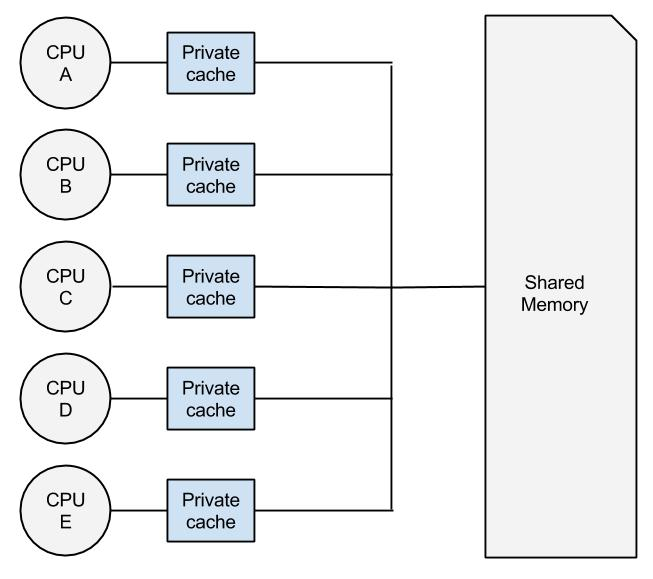
\includegraphics[width=1\textwidth]{img/Tightly Coupled Multi-Processing Systems.jpg}
        \caption{An Example of Tightly Coupled Multi-Processing Systems}
        \label{fig:tightlycoupled}
    \end{figure}
Tightly coupled multi-processing systems have many processor with their own caches and one shared memory\cite{Jim2007}. Cache memories are not developed with same purpose with memories, but they are developed for performance reason which we discussed in background studies. If we exploit them and design our program properly, cache memories could behave as another layer of memories, and on the monitoring side, even if it perfectly scan memories and detect malicious codes, cache memories are still out of the box.

The required systems for our technique in this chapter is tightly coupled multi-processing systems without cache coherence interconnector. Also, we need simple Harvard computer architecture instead of Von Neumann. Incoherent systems are surprisingly popular because of the implementation errors i.e. Samsung's mainstream CPU Exynos 5410 which sold millions, and also due to costs. Many hardware designers also believe programming with shared memory is not appropriate way and platforms such as Android already using message based communication on multi-threaded application, and  they implement clustered processors which limits programs instead of implementing expensive coherency interconnector. Yet they do not consider security approaches.

	

	\section{Exploiting Tightly Coupled Multi-Processing Systems}
	    \begin{figure}[h!]
	        \centering
	        \includegraphics[width=1\textwidth]{img/attack vector.jpg}
	        \caption{Attack vector flow chart}
	        \label{fig:atackvector}
	    \end{figure}
	    In this section, we will formulate our attack vector one by one, and we will show implementation and theoretical obstacles. Essence of the thesis is exploiting caches to hide values from upper layer memories but also it concern some subtle studies to run a comprehensive code from beginning to end. In figure \ref{fig:atackvector}, our attack vector flow chart showed. There is no doubt that most important part of our attack is designing and reconnaissance part, because after we produce cache oriented malware, it is a kind of system depended malware and can't work on the every systems, but can be useful as targeted attacks (e.g Stuxnet). Targeted attacks could be really efficient because of the facts that, all anti malware tools aims massive market, and if malware aims sneakily small portion of the market, they could be successful forever. Setting system up and loading memory second step of the attack vector and first step of attack loop. In this section, we will show cache tricks and explain why it is efficient. In the last chapter we will emphases obfuscation and deobfuscation methods briefly, and we will discuss some control flow issues. As you can see, when code or data is deobfuscated, it is on the cache memory. When we call the next independent part of the code, it must definitely be obfuscated back, because we do not want to evict cache blocks to memory plain. 
	    \subsection{Reconnaissance and Design}
	    Design and reconnaissance is the most crucial part of our attack approach, because the size of the cache memory is the basic dependence. If you try to fill more data than its actual size to cache memory, it evicts a number of cache blocks depending on the replacement policy. It is what really we do not want, if the evicted block are not obfuscated. Our first design approach to prevent leakage of plain data upper layer of the cache memory. As we have seen in background chapter, cache are a kind of memories but it also comprise with logical circuit to replace its block autonomously, because they are incomparably small and depending on the main memory to store and load informations. If we claimed they are invisible layer between memory and processors, it would not be totally wrong, and also many programmers today do not concern about their performance feature when they design their program's loops. On the other side, if you consider cache properties while designing your programs, It is hard to determine the base system. For example if we have 32 byte cache block, we could consider when we load an address it will load 32 byte into the cache and in the most frequently working look could progress on this values e.g. arrays are continues bytes and they are generally loading all together. However, cache sizes are extremely various today on the market and if you design a cache oriented program for 32 byte cache block it will not work properly on the cache which has 20 cache block size. Beside that fact, cache size is also important constraint and worst, they have more various then cache block size on the market.

	    Therefore, we propose to generate a specific piece of code to fit for each cache corresponding to cache size, cache characteristic and also target system  arch and security level. Target system architecture may imply cache architecture, and we could design more complex and more flex gadget with multi layer cache arch. if many processors can reach a cache and share values, we could easily broke control flow graph\cite{ramilli2011multiprocess}, and also on the higher level caches we should use more memory space comparing with lower layer, but if and only if there is no malware sensor which is monitoring memory, we should use upper layer of memory. When we are using a CPU, it is quite certain that it is the only one who is accessing corresponding cache. In figure \ref{fig:gadgetsections}, illustration of a gadget is showed. It has two sections which are stub and body. This body section is loaded with actual gadget code and tail section. Tail section is responsible with stitching gadget properly. So every gadgets knows before they started to run, which gadget they are followed by. It is a bit problematic and tricky, see Pitfalls and Fallacies section for details.

	    When we determine the gadgets size, we should consider the cache properties, such as replacement policy, block size, set associativity, line size and total size of cache. The size of gadget must not be more than the total size of cache, and also must be designed with no eviction before obfuscation principles. Hence, we must know who will be evicted next always. On random eviction model, we should not consider eviction during processing of gadget. During running a gadget code, also we must be sure there is memory load or store operation to memory except gadget memory space. Also all gadget must be adjusted to settle in memory continuously in order to utilize spacial locality.

	    \begin{figure}[h!]
	        \centering
	        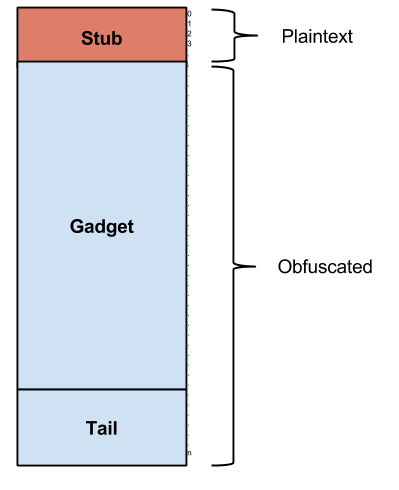
\includegraphics[width=0.5\textwidth]{img/Code_illustration.png}
	        \caption{Gadget Sections}
	        \label{fig:gadgetsections}
	    \end{figure}

 	    \subsection{Setting system up and Loading Cache Memory}
\begin{lstlisting}
	mov r2, 0x012345 #address
	mov r3, 0x013456 #end of gadget
	mov r4, 0 #counter
fetch: 	addi r2, r4 # add size of word to address
	mov r1, [r2] #Load address from memory
	cmp r2,r3 # compare r2 and r3
	jl fetch
\end{lstlisting}
	    \subsection{Obfuscating Running and Deobfuscating gadget}
	


	\section{Pitfalls and Fallacies}
		It is a bit tricky because it constrains functional programming, because you can not use gadgets as functions and it is really usual for functions to be independent from rest of the part, it makes them good candidate to be gadgets. Therefore, we must implements a function again and again for each use to convert them the obfuscated gadgets. However, designing malware with almost every feature it can have does not book even several megabytes.
		Write Through caches
		Coherency Mechanism
		Harvard Arch
		Caches are not memory
		Context switching